
\chapter{Sperimentazioni}
\label{chap:sperim}
In questo capitolo verranno riportati i risultati osservati nella fase di classificazione dei dataset ottenuti dalle features dai file audio splittati, ottenuti a partire dalle applicazioni Andorid. Da prima vedremo come sono composti i dataset ed in seguito quali sono i risultati ottenuti dalle classificazioni. Il processo di addestramento di modelli di multiple instance learning è avvenuto attraverso l'utilizzo del software WEKA [\ref{par:weka}]. 
La bontà delle classificazioni effettuate si è calcolata dalle due metriche precision e recall sopra descritte [\ref{par:precisionRecall}]. Nel processo di training di ogni modello di classificazione utilizato si è impiegato l'utilizzo della K-Fold Validation [\ref{par:kfold}], nel dettaglio la divisione e ripetizione è avvenuta sul 10\% del dataset, impostando il valore $K = 10$, di conseguenza i valori di precision e recall rappresentano la media aritmetica delle 10 iterazioni eseguite durante l'addestramento.
\section{Classificazione multi classe}
Come detto in precedenza, al paragrafo \ref{par:datasetApk}, le applicazioni utilizzate provengono da due dataset "trusted" e "Acid". Le applicazioni Acid dono di diverso tipo, ”broadcast\_intent”, ”shared\_preferences” o ”external\_storage”. Dopo aver effettuato una prima conversione delle applicazioni Android in file audio di tipo wav, lo splitting degli stessi è stato effettuato in due passaggi. Nella prima operazione di splitting, la suddivisione è stata effettuata in intervalli di circa  35 minuti (2092 secondi) ricavando quindi dall'estrazione delle feature da ogni file audio suddiviso, un dataset "\textit{data\_2092.arff}" di 682 bag, il maggior numero delle quali composte da circa 8 istanze. Nella seconda operazione di splitting, la suddivisione è stata effettuata in intervalli di circa 17 minuti (1046 secondi) in questo modo il numero di bag che vanno a comporre il dataset "\textit{data\_1046.arff}" è come prima di 682 bag, la maggior parte delle quali popolata però da 16 istanze.
In figura \ref{fig:multiclassdataset} si può osservare la suddivisione delle classi. 
\begin{figure}[h]
\centering
    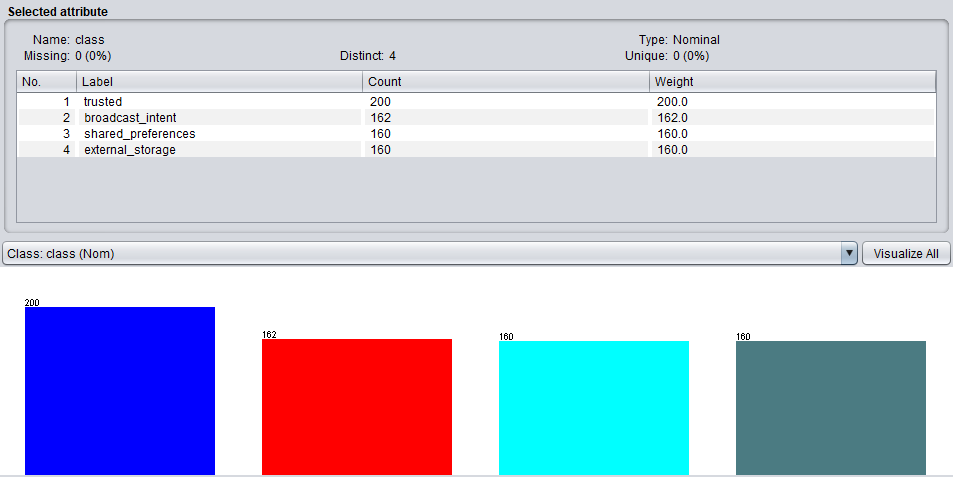
\includegraphics[width=0.9\linewidth]{imgs/capitolo5/multicalsse/682 bag 4 classi.png} 
    \caption{Multi class dataset}
    \label{fig:multiclassdataset}
\end{figure}
\FloatBarrier
La classificazione è stata eseguita adottando il criterio della K-Fold validation [\ref{par:kfold}].
Nello specifico l'algoritmo utilizzato è stato il TLC che ha restituito per il dataset "\textbf{data\_2092.arff}":
\begin{itemize}
    \item Precision: 0.847 
    \item Recall: 0.845
\end{itemize}
mentre per il dataset "\textbf{data\_1046.arff}" i valori osservati sono:
\begin{itemize}
    \item Precision: 0.844 
    \item Recall: 0.845
\end{itemize}

In figura \ref{fig:plotMulticlasse} si può osservare come le istanze del test set sono state classificate. Nello specifico sulle ascisse è riportata la classe predetta dal modello mentre sulle ordinate la classe di appartenenza originale. Alle istanze è stata applicata Jitter per una migliore visualizzazione. Le istanze rappresentate da una 'x' sono state predette correttamente, ovvero la classe coincide con la classe predetta dal modello, mentre le classi rappresentate dal quadratino sono quelle istanze erroneamente classificate dal modello, la cui classe d'appartenenza è la corrispondete sull'asse delle ordinate che da anche il colore alle istanze, mentre la predetta è la classe corrispondete sulle ascisse. 
\begin{figure}[h]
\centering
    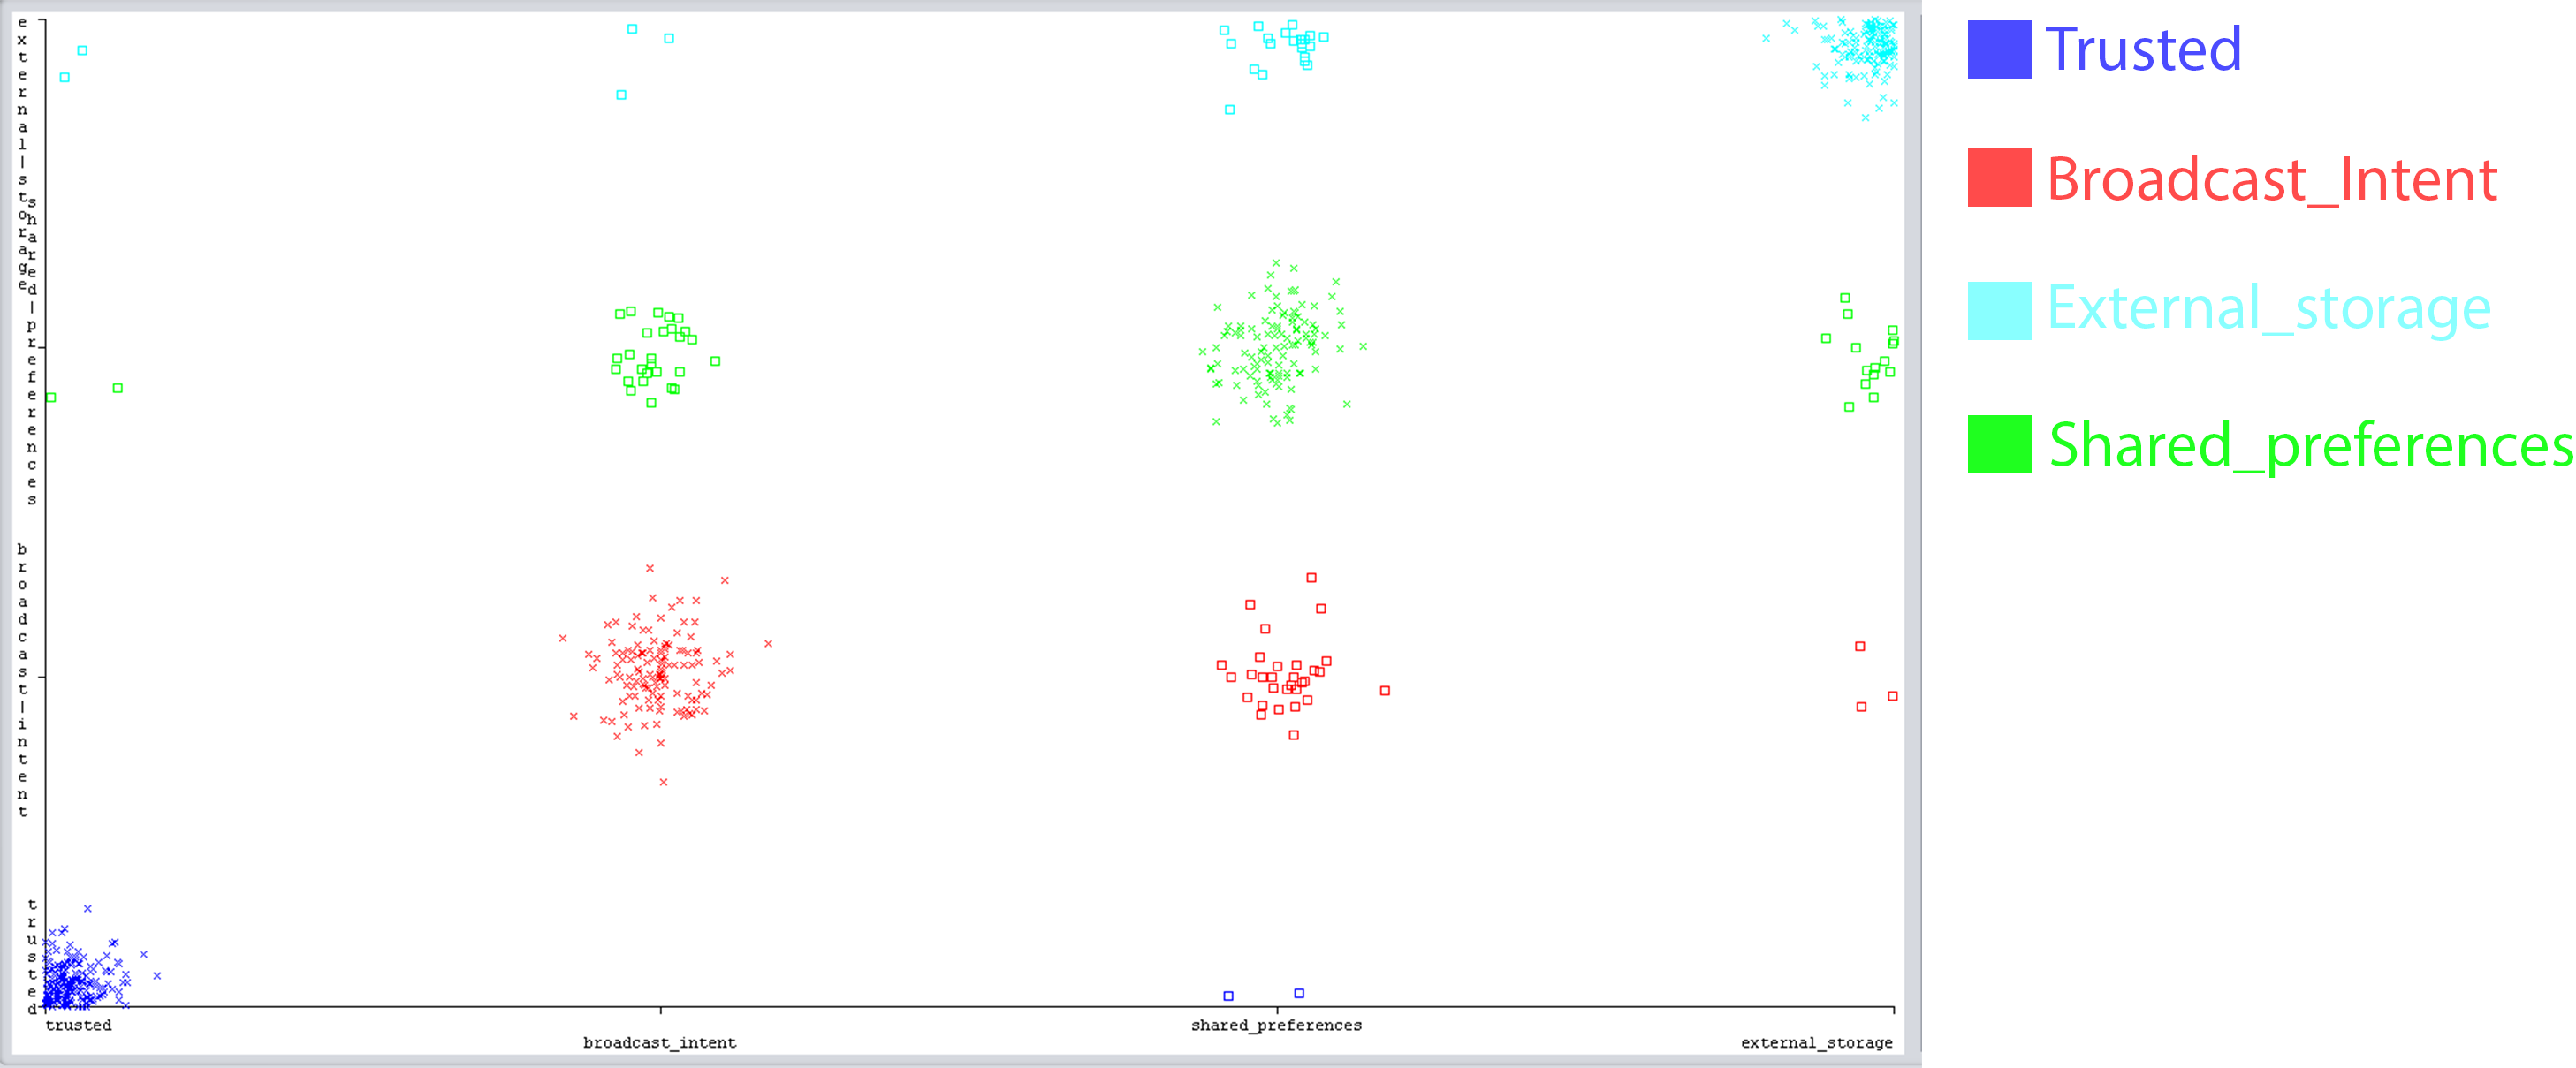
\includegraphics[width=0.9\linewidth]{imgs/capitolo5/multicalsse/data_multiclass_visual.png} 
    \caption{Multi class classification}
    \label{fig:plotMulticlasse}
\end{figure}
\FloatBarrier

\section{Classificazione binaria Trusted - Malware}
La seconda sperimentazione effettuata riguarda la classificazione dei dataset le cui classi d'appartenenza sono "trusted" e "malware". I dataset popolati da 682 bag sono stati ricavati da istanze di audio splittati in circa  35 minuti (2092 secondi) da cui si è ottenuto il dataset "dataBinary\_2092.arff" e da audio suddivisi in intervalli di circa 17 minuti (1046 secondi) da cui abbiamo ricavato il dataset "dataBinary\_1046.arff". Le classi delle bag sono composte da 200 bag con label "trusted" e 482 bag con label "malware" come si può osservare dall'istogramma in figura \ref{fig:bindataset}.
\begin{figure}[h]
\centering
    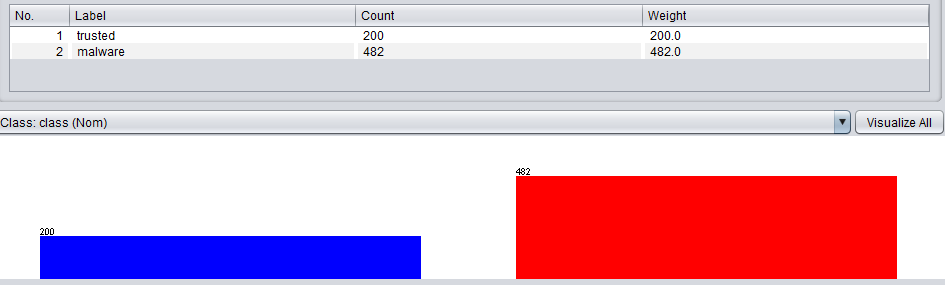
\includegraphics[width=0.9\linewidth]{imgs/capitolo5/multicalsse/binaryclass.png} 
    \caption{Binary class dataset}
    \label{fig:bindataset}
\end{figure}
\FloatBarrier

Le classificazioni hanno riguardato diversi algoritmi, i risultati, valutati attraverso i valori di precision e recall sono stati: 

\begin{center}
 \begin{tabularx}{0.8\textwidth} { | >{\raggedright\arraybackslash}X | >{\centering\arraybackslash}X | >{\raggedleft\arraybackslash}X | }
        \hline
        \multicolumn{3}{|c|}{\textbf{Dataset dataBinary\_2092}}\\
        \hline
       \textbf{ALG} & \textbf{PRECISION} & \textbf{RECALL} \\
       \hline
       MIEMDD  & 0.999  & 0.999  \\
        \hline
       MIDD   & 0.997  & 0.997  \\
        \hline
       QUICK DD  & 0.996  & 0.996  \\
        \hline
       TLC  & 0.993  & 0.993  \\
        \hline
       MITI  & 0.981  & 0.981  \\
        \hline
       MIRI  & 0.980  & 0.979  \\
        \hline
       MILR  & 0.949  & 0.946  \\
        \hline
       CitationKNN  & 0.924  & 0.915  \\
       \hline
       MDD  & 0.852 & 0.818  \\
        \hline
       MISVM  & 0.806  & 0.733  \\
        \hline
       TLD  & 0.79  & 0.299  \\
       \hline
    \end{tabularx}
    \end{center}
\begin{center}
    
    %%secodna tabella%%
 \begin{tabularx}{0.8\textwidth} { | >{\raggedright\arraybackslash}X | >{\centering\arraybackslash}X | >{\raggedleft\arraybackslash}X | }
        \hline
        \multicolumn{3}{|c|}{\textbf{Dataset dataBinary\_1046}}\\
        \hline
       \textbf{ALG} & \textbf{PRECISION} & \textbf{RECALL} \\
       \hline
       MIEMDD  & 0.997  & 0.997  \\
        \hline
             TLC  & 0.996  & 0.996  \\
        \hline
         QUICK DD  & 0.991  & 0.991  \\
        \hline
       MITI  & 0.913  & 0.902  \\
        \hline
       MIRI  & 0.913  & 0.902  \\
        \hline
       MILR  & 0.981  & 0.981  \\
        \hline
       CitationKNN  & 0.916  & 0.905  \\
       \hline
       MDD  & 0.915 & 0.905  \\
        \hline
       MISVM  & 0.802  & 0.724  \\
        \hline
        \end{tabularx}
\end{center}

Dunque il risultato migliore si è ottenuto con l'algoritmo MIEMDD in entrambi i dataset. 

\section{Classificazione binaria Apk\_Get - Apk\_Put}
In questa sperimentazione, i dataset comprendono solo le applicazioni affette da malware provenienti dal dataset "Acid". Le bag di ogni dataset sono quindi in totale 482, suddivise in due classi Apk\_Get e Apk\_Put come descritto nel paragrafo \ref{par:dataset}. 
Nella figura \ref{fig:getputclassdataset} possiamo osservare l'istogramma relativo alle due classi sopra descritte. 
\begin{figure}[h]
\centering
    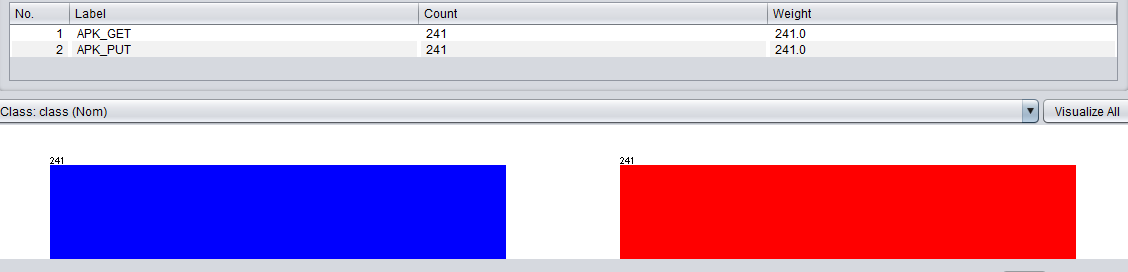
\includegraphics[width=0.9\linewidth]{imgs/capitolo5/multicalsse/getputclass.png} 
    \caption{Get - Put class dataset}
    \label{fig:getputclassdataset}
\end{figure}
\FloatBarrier

Anche in questo caso la classificazione ha ricoperto l'utilizzo di più algoritmi. La classificazione è stata eseguita sui due dataset "dataGetPut\_2092.arff" e "dataGetPut\_1046.arff" e la valutazione eseguita sulla bontà dei risultati di precision e recall. I valori osservati sono stati i seguenti: 
\begin{center}
 \begin{tabularx}{0.8\textwidth} { | >{\raggedright\arraybackslash}X | >{\centering\arraybackslash}X | >{\raggedleft\arraybackslash}X | }
        \hline
        \multicolumn{3}{|c|}{\textbf{Dataset dataGetPut\_2092}}\\
        \hline
       \textbf{ALG} & \textbf{PRECISION} & \textbf{RECALL} \\
       \hline
       TLC  & 0.979  & 0.979  \\
        \hline
       MITI   & 0.971  & 0.971  \\
        \hline
       MIRI  & 0.965  & 0.965  \\
        \hline
       MIDD  & 0.878  & 0.861  \\
        \hline
       MDD  & 0.804  & 0.712  \\
        \hline
       TLDSIMPLE  & 0.755  & 0.519  \\
        \hline
       MIEMDD  & 0.751  & 0.502  \\
        \hline
       QUICKDD  & 0.729  & 0.726  \\
       \hline
       MILR  & 0.599 & 0.562  \\
        \hline
       BOOST  & 0.498  & 0.498  \\
        \hline
       WRAPPER  & 0.498  & 0.498  \\
       \hline
        CitationKNN  & 0.497  & 0.498  \\
       \hline
        SIMPLEMI  & 0.494  & 0.498  \\
       \hline
    \end{tabularx}
    \end{center}
\begin{center}
    
    %%secodna tabella%%
 \begin{tabularx}{0.8\textwidth} { | >{\raggedright\arraybackslash}X | >{\centering\arraybackslash}X | >{\raggedleft\arraybackslash}X | }
        \hline
        \multicolumn{3}{|c|}{\textbf{Dataset dataGetPut\_1046}}\\
        \hline
         \textbf{ALG} & \textbf{PRECISION} & \textbf{RECALL} \\
       \hline
       TLC  & 0.992  & 0.992  \\
        \hline
       MITI   & 0.979  & 0.979  \\
        \hline
       MIRI  & 0.975  & 0.975  \\
        \hline
       MIDD  & 0.913  & 0.913  \\
        \hline
       MDD  & 0.805  & 0.703  \\
        \hline
       TLDSIMPLE  & 0.754  & 0.515  \\
        \hline
       MIEMDD  & 0.700  & 0.618  \\
        \hline
       QUICKDD  & 0.869  & 0.838  \\
       \hline
       MILR  & 0.574 & 0.573  \\
        \hline
       BOOST  & 0.498  & 0.498  \\
        \hline
       WRAPPER  & 0.498  & 0.498  \\
       \hline
        CitationKNN  & 0.497  & 0.498  \\
       \hline
        SIMPLEMI  & 0.494  & 0.498  \\
       \hline
        \end{tabularx}
\end{center}
Nel classificare questi dataset il risultato migliore è stato ottenuto con l'utilizzo dell'algoritmo TLC. 